\documentclass[letterpaper, reqno,11pt]{article}
\usepackage[margin=1.0in]{geometry}
\usepackage{color,latexsym,amsmath,amssymb,graphicx, float}
\usepackage{hyperref}

\hypersetup{
colorlinks=true,
linkcolor=magenta,
filecolor=magenta,
urlcolor=cyan,
}

\graphicspath{ {images/} }

\begin{document}
\pagenumbering{arabic}
\title{ELEC 481 Homework 9}
\date{24/06/22}
\author{Xander Naumenko}
\maketitle

{\noindent\bf Question 1.} See figure \ref{fig:q1}. The return for bonds was calculated using $(1+i/n)^n$, and stocks have no tax break. Using excel the WACC was calculated to be 9.2\% and after tax it was 7.91\%. 

\begin{figure}[htpb]
    \centering
    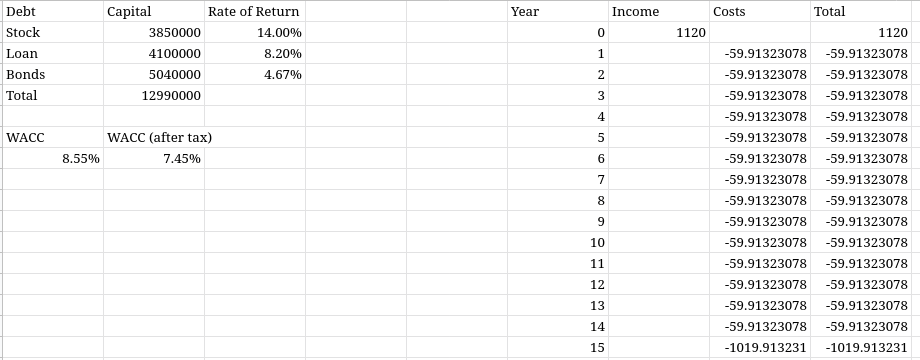
\includegraphics[width=0.8\textwidth]{q1}
    \caption{WACC analysis for question 1}
    \label{fig:q1}
\end{figure}

{\noindent\bf Question 2a.} The total tax will be 

\[
t=45282\cdot 0.15+(90563-45282)\cdot 0.205+(140388-90563)\cdot 0.26+(200000-140388)\cdot 0.29+
\]
\[
20000\cdot 0.33-11474\cdot 0.15=\$51195.78
.\]

{\noindent\bf Question 2b.} Personal: 

\[
t=45282\cdot 0.15+(90563-45282)\cdot 0.205+(130000-90563)\cdot 0.26-11474\cdot 0.15=\$24607
.\]

The corporate tax would be: 
\[
t=90000\cdot 0.15=\$13500
.\]

The total would then be $\$38107$. 

\begin{figure}[htpb]
    \centering
    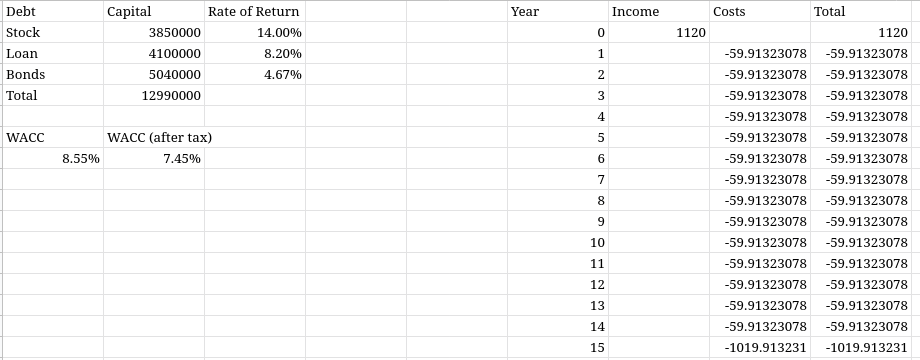
\includegraphics[width=0.8\textwidth]{q1}
    \caption{WACC calculations for question 1}
    \label{fig:q1}
\end{figure}

{\noindent\bf Question 2c.} Yes she should, as the total cost of taxes is lower. The amount of money saved is $51195.78-38107=\$13089$

{\noindent\bf Question 3a.} See figure \ref{fig:q3} for the completed table using excel. From the table we see that the book value when the equipment is sold would be: 

\[
BV=60000-16500-23925-10766.3-4844.8=\$3963.9
.\]

{\noindent\bf Question 3b.} Since the equipment was sold for more than its book value, it is a recaptured depreciation. The amount of gain is $8000-3963.9=\$4036.1$. 

\begin{figure}[htpb]
    \centering
    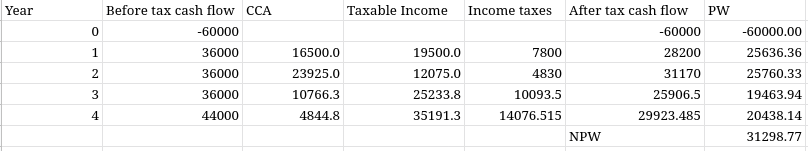
\includegraphics[width=0.8\textwidth]{q3}
    \caption{Cash flow table for question 3}
    \label{fig:q3}
\end{figure}

{\noindent\bf Question 3c.} From the table the net present worth at the end of the situation is \$28591.38, since this is above \$0 which is the do nothing alternative, it was a good decision. 

{\noindent\bf Question 4a.} See figure \ref{fig:q4}, there the running EUAC is calculated for each year. This was done using the gradient value depreciation formula: 

\[
    (G/A, i, n)=\left( \frac{1}{i}-\frac{n}{(1+i)^{n}-1} \right) 
.\]
Based on this we see that the EUAC after 10 years is \$4327.44. 

\begin{figure}[htpb]
    \centering
    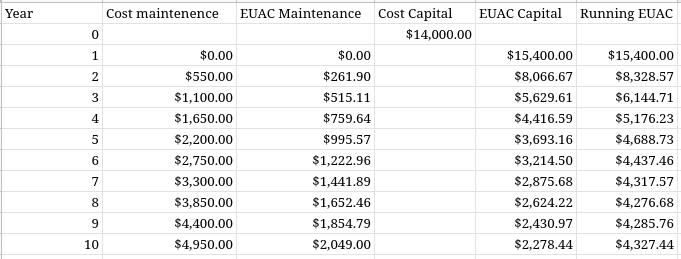
\includegraphics[width=0.8\textwidth]{q4}
    \caption{Cost analysis for question 4a}
    \label{fig:q4}
\end{figure}

{\noindent\bf Question 4b.} Looking at the table, we see that the minimum cost is in year 8. 

{\noindent\bf Question 4c.} To minimize the cost of the machine we want to minimize the EUAC, so it would make sense to get rid of it and replace it after year 8, i.e. after year 8 and before year 9. However this doesn't take into account any money that would result from selling, which would change the analysis. 

\end{document}
